\documentclass{beamer}

\usepackage[utf8]{inputenc}
\usetheme{Singapore}
\usepackage{xcolor}
\setbeamertemplate{footline}[frame number]

\usepackage{mathlist}

\usepackage[francais]{babel}
\usepackage{amsmath,amssymb}

\newtheorem{theo}{Théorème}

\usepackage{times}

\usepackage{ulem, pstricks}

\usepackage{listings}
%\topmargin=-0.6in
\lstloadlanguages{C++}
\lstset{language=C++}
%%}

\setbeamercovered{dynamic}

\def\bxi{\boldsymbol\xi}
\def\bomega{\boldsymbol\omega}

\def\cK{\mathcal{K}}
\def\cB{\mathcal{B}}
\def\cQ{\mathcal{Q}}


\title[$L$-shaped method]{Stochastic optimization\\$L$-shaped method}

\author[Fabian Bastin]{Fabian Bastin\\\url{fabian.bastin@polymtl.ca}\\Université de Montréal -- CIRRELT}

\date{}

\begin{document}

\frame{\titlepage}

\begin{frame}
\frametitle{Two-stage linear program with recourse}

{\red Suggested reading: Section~3.2, Kall et Wallace}

\mbox{}

Summarize our formulations.
\[
\min_{x \in \rit^n_+ \,|\, Ax = b} \left\lbrace c^Tx + E_{\bxi} \left[ \min_{y \in \rit^p_+} \lbrace q(\bxi)^Ty \ |\ Wy = h(\bxi) - T(\bxi)x \rbrace \right] \right\rbrace 
\]
\[
\min_{x \in \rit^n_+ \,|\, Ax = b} \left\lbrace c^Tx + E_{\bxi}
  \left[  v(\bxi, h(\bxi)-T(\bxi)x) \right] \right\rbrace 
\]
\[
\min_{x \in \rit^n_+ \,|\, Ax = b} \left\lbrace c^Tx + E_{\bxi} \left[ Q(x,\bxi) \right] \right\rbrace 
\]
\[
\min_{x \in \rit^n_+} \left\lbrace c^Tx + \mathcal{Q}(x)
  \ |\ Ax = b \right\rbrace 
\]

We have studied its properties. But how to solve it?

\end{frame}

\begin{frame}
\frametitle{Notations: reminder}

\begin{itemize}
\item
First-stage feasible set:
\[
K_1 = \lbrace x \in \rit^n_+ \ |\ Ax = b \rbrace.
\]
\item
Second-stage feasible set:
\[
K_2 = \lbrace x \ |\ \mathcal{Q}(x) < \infty \rbrace.
\]
\end{itemize}
We can therefore rewrite the problem as
\[
\min_x \lbrace c^Tx + \mathcal{Q}(x) \ |\ x \in K_1 \cap K_2 \rbrace.
\]

%\mbox{}

%For simplicity, we will assume for now that the recourse is relatively complete.

\end{frame}

\begin{frame}
\frametitle{Deterministic equivalent}

Assume now that the support of $\bxi$ is finite, and that we have $S$ scenarios.
The probability of scenario $s$ is $p_s$.

\mbox{}

The deterministic equivalent is
\begin{align*}
\min_{x \in X, y_1, \ldots, y_S}\ & c^T x + p_1 q^T y_1 + p_2 q^T y_2 + \ldots
p_S q^Ty_S \\
\mbox{s.t. } & \\
& \begin{matrix} Ax & & & & & = b\\
T_1 x & + W y_1 & & & & = h_1 \\
T_2 x & & + W y_2 & & & = h_2 \\
\vdots & & & \ddots & \\
T_S x & & & & + W y_S & = h_S
\end{matrix} \\
& x \in X,\ y_1 \in Y,\ y_2 \in Y,\ldots, y_S \in Y.
\end{align*}

\end{frame}

\begin{frame}
\frametitle{Properties of the deterministic equivalent}

\begin{itemize}
\item
$y_s \overset{def}{=} y(\omega_s)$ is the recourse action to take if the scenario $s$ occurs.
\item
We obtain a linear program,\ldots but very large:
\begin{itemize}
\item
n + pS variables;
\item
m1 + mS constraints.
\end{itemize}
\item
The constraints has a very specific structure (staircase).
\item
{\red Idea}: use decomposition techniques.
\end{itemize}

\end{frame}

\begin{frame}
\frametitle{Decomposition methods}

{\red General principle}: the nonlinear term (the recourse function) implies to compute the solution of all the second-stage recourse linear programs.

\mbox{}

Is is possible to avoid repeated evaluations of all the concerned functions in order to compute these solutions?

\mbox{}

{\red Idea}: build a master program in $x$, and evaluate the objective function exactly (including all the scenarios) as a subproblem only.

\end{frame}

\begin{frame}
\frametitle{Block structure}

\begin{minipage}{0.49\textwidth}
Primal:
$$
\begin{pmatrix}
A \\
T_1 & W \\
T_2 & & W \\
\vdots & & & \ddots \\
T_S & & & & W
\end{pmatrix}
$$
\end{minipage}
\begin{minipage}{0.49\textwidth}
Dual:
	$$
	\begin{pmatrix}
	A^T & T_1^T & T_2^T & \cdots & T_S^T \\
	& W^T \\
	& & W^T \\
	& & & \ddots \\
	& & & & W^T
	\end{pmatrix}
	$$
\end{minipage}

\mbox{}

The figures have give the name to the method: L-shaped.
\end{frame}

\begin{frame}
\frametitle{Main ideas}

{\red Section 1.6.4, Kall and Wallace}

Assume for now that $\Xi$ contains one element only.
The problem becomes
\begin{align*}
\min_{x,y}\ & c^Tx + q^Ty & \\
\mbox{s.t. } & Ax = b, \\
& Tx + Wy = h, \\
& x \geq 0,\ y \geq 0.
\end{align*}

\mbox{}

The problem can be reformulated as
\begin{align*}
\min_x\ & c^Tx + f(x) \\
\mbox{s.t. } & Ax = b, x \geq 0,
\end{align*}
with
\[
f(x) \overset{def}{=} \min_y \lbrace q^Ty \ |\ Wy = h - Tx,\ y \geq 0 \rbrace.
\]

\end{frame}

\begin{frame}
\frametitle{Problem reformulation}

Assume moreover that the problem is feasible and $\lbrace x \,|\, Ax = b,\ x \geq 0 \rbrace$ is bounded. This implies that
\[
\inf \lbrace f(x) \ |\ Ax = b,\ Tx+Wy =h,\ x \geq 0 \rbrace
\]
is finite and $f(x)$ can be uniformly bounded from below on $K_1$, say by $\theta$.

\mbox{}

If we explicitly know $f(x)$, we can write
\begin{align*}
\min_x\ & c^Tx + f(x) & \\
\mbox{t.q. } & Ax = b, \\
& \theta - f(x) \geq 0, \\
& x \geq 0.
\end{align*}

\end{frame}

\begin{frame}
\frametitle{First ideas}

Try to construct a {\blue sequence of new (additional) linear constraints} in order to define a feasible $\mathcal{B}_1$ of vectors $(x_1,\ldots,x_n,\theta)^T$ in $\rit^{n+1}$, such that, with
\[
\mathcal{B}_0 = \lbrace (x^T, \theta^T) \,|\, Ax = b,\ x \geq 0,\
\theta \in \rit \rbrace,
\]
the problem
\[
\min_{(x,\theta) \in \mathcal{B}_0 \cap \mathcal{B}_1} c^Tx+\theta
\]
gives a (first-stage) solution of the initial problem and an estimation $\theta$ of the second-stage objective value.

\end{frame}

\begin{frame}
\frametitle{Dual decomposition method}

\begin{description}
\item[\red Step 1]
Let $\theta_0$ be a lower bound for
\[
\min_y \lbrace q^Ty \,|\, Ax = b,\ Tx+Wy = h,\ x \geq 0,\ y \geq 0 \rbrace,
\]
and let $(\hat{x}, \hat{\theta})$ be a solution of
\[
\min_x \lbrace c^Tx + \theta \,|\, Ax = b,\ \theta \geq \theta_0,\ x
\geq 0 \rbrace.
\]
Set also $\mathcal{B}_1 := \lbrace \rit^n \times \lbrace \theta \rbrace
\,|\, \theta \geq \theta_0 \rbrace$.
\item[\red Step 2]
Evaluate
\begin{align*}
f(\hat{x}) &= \min_y \lbrace q^Ty \,|\, Wy = h-T\hat{x},\ y \geq 0
\rbrace \\
&= \max_u \lbrace (h-T\hat{x})^Tu \,|\, W^Tu \leq q \rbrace. \mbox{ (duality)}
\end{align*}
We have to consider two cases.
\end{description}
\end{frame}

\begin{frame}
\frametitle{Dual decomposition method (cont'd)}

{\red Step 2 (a)}
If $f(\hat{x}) = +\infty$, $\hat{x}$ is not feasible with all the second-stage constraints, there is no $y$ satisfying the linear system.

\mbox{}

\begin{block}{Farkas' lemma}
Let $A \in \rit^{m \times n}$ and $b \in \rit^m$.
Then, exactly one of the following two statements is true:
\begin{itemize}
\item
$\exists\, x \in \rit^n$ such that $Ax = b$ and $x \geq 0$;
\item
$\exists\, u \in \rit^m$ such that $u^T A \geq 0$ and $u^T b < 0$;
\end{itemize}
\end{block}
	
\mbox{}

Therefore, if $y$ is not feasible, $\exists$ $\tilde{u}$ such that
\[
-W^T\tilde{u} \geq 0 \mbox{ et } (h - T\hat{x})^T \tilde{u} < 0.
\]
or
\[
W^T\tilde{u} \leq 0 \mbox{ et } (h - T\hat{x})^T \tilde{u} > 0.
\]

\end{frame}

\begin{frame}
\frametitle{Dual decomposition method (cont'd)}

Now, given $x$ feasible (for the first and second stage), there exists $y \geq 0$ s.t. $Wy = h-Tx$.
For such a $y$, we have
\[
\tilde{u}^T(h-Tx) = \tilde{u}^T W y \leq 0.
\]
as $W^T\tilde{u} \leq 0$ and $y \geq 0$.
Therefore
\[
\tilde{u}^Th \leq \tilde{u}^TTx.
\]
This inequality should be valid for any feasible $x$ (therefore excluding $\hat{x}$), and we will enforce it by adding it to the first-stage linear program: {\red feasibility cut}
\[
\tilde{u}^T(h-Tx) \leq 0.
\]
Redefine $\mathcal{B}_1 := \mathcal{B}_1 \cap \lbrace (x^T,
\theta) \,|\, \tilde{u}^T(h-Tx) \leq 0 \rbrace$.

\end{frame}
%	\mbox{}
	
%	Recours relativement complet: $z \in \mbox{pos} W$ ou $\lbrace y \,|\,
%	Wy = z,\ y \geq 0\rbrace \ne \emptyset$.
	
%	Par le lemme de Farkas, cela équivaut à
%	$(W^Tu \geq 0) \Rightarrow (z^Tu \geq 0).$
	

\begin{frame}
\frametitle{Dual decomposition method (cont'd)}

{\red Step 2 (b)}
If $f(\hat{x})$ is finite, given $\hat{x}$, we have a primal optimal solution $\hat{y}$ and a dual optimal solution $\hat{u}$ with
\[
f(\hat{x}) = (h-T\hat{x})^T \hat{u}
\]
by the strong duality property.

\mbox{}

Moreover, for any $x$, we can write
\begin{align*}
f(x) &= \sup_u \left\lbrace (h-Tx)^Tu \,|\, W^Tu \leq q \right\rbrace \ \mbox{(second stage dual)}\\
&\geq (h-Tx)^T \hat{u} \\
&= \hat{u}^T(h-Tx).
\end{align*}

Since we want $\theta$ to represent $f(x)$, we would like
\[
\theta \geq \hat{u}^T(h-Tx).
\]

\end{frame}

% nous avons une solution optimale primale de base $\hat{y}$ et une solution optimale
% duale basique $\hat{u}$, avec

\begin{frame}
\frametitle{Dual decomposition method (cont'd)}

$\theta \geq \hat{u}^T(h-Tx)$ is violated at $(\hat{x}, \hat{\theta})^T$
iff $\hat{u}^T(h-T\hat{x}) > \hat{\theta}$.

In this case we introduce the optimality cut, rejecting the suboptimal solution $(\hat{x}^T, \hat{\theta})^T$:
\[
\theta \geq \hat{u}^T (h-Tx),
\]
and we redefine $\mathcal{B}_1 := \mathcal{B}_1 \cap \lbrace (x^T,
\theta) \,|\, \theta \geq \hat{u}^T (h-Tx) %\leq 0 ???
\rbrace$.

\mbox{}

If $f(\hat{x}) \leq \hat{\theta}$, stop: $\hat{x}$ is a first-stage solution.
Otherwise, go to Step 3

\mbox{}

{\red Step 3}
Solve the updated problem
\[
\min \lbrace c^Tx + \theta \,|\, (x^T, \theta) \in \mathcal{B}_0 \cap
\mathcal{B}_1 \rbrace.
\]
Return to Step 2 with the new solution $(\hat{x}, \hat{\theta})$.

\end{frame}

\begin{frame}
\frametitle{Convergence}

{\blue Stopping rule}: $f(\hat{x}) \leq \hat{\theta}$.

Since
\begin{align*}
\hat{\theta} &= \max_{1 \leq i \leq k} (h-T\hat{x})^Tu^i
\leq \max_{1 \leq i \leq r} (h-T\hat{x})^Tu^i \\
&= f(\hat{x}) \leq \hat{\theta},
\end{align*}
the algorithm stops for $\hat{\theta}$ optimal.


\begin{block}{Proposition}
If the two-stage stochastic program is solvable and $\lbrace x
\,|\, Ax=b,\ x \geq 0 \rbrace$ is bounded, the dual decomposition method gives an optimal solution after a finite number of iterations.
\end{block}

\end{frame}

\begin{frame}
\frametitle{$S$ scenarios}

If $\Xi$ is finite, but is not a singleton?

\mbox{}

We can introduce feasibility and optimality cuts for all the recourse functions
\[
Q_{s}(x) = \min \left\lbrace (q_{s}^T y_{s} \,|\, Wy_{s} = h_{s}-T_{s}x,\ y_{s} \geq 0 \right\rbrace,
\]
$s = 1,\ldots,S$.
We obtain a {\sl \red multi-cut} dual decomposition method

\mbox{}

Alternatively, we can combine cuts corresponding to blocks $s = 1,\ldots,S$ with their respective probabilities.

\end{frame}

\begin{frame}
\frametitle{Single-cut algorithm}
	
For $S$, we can proceed as before, by remplacing $\mathcal{Q}(x)$ by $\theta$: singe-cut.
This leads to the {\red master program}
\begin{align*}
	\min c^Tx & + \theta \\
	\mbox{t.q. } Ax & = b, \\
	\theta &\geq \mathcal{Q}(x),\\
	x & \geq 0,\ \theta \in \rit.
\end{align*}
This program has $n+1$ variables only!

%\mbox{}

%Alternatively, we can consider cuts for a disjoint subsets of alternatives: multi-cut. We will consider this version later.

\end{frame}

\begin{frame}
\frametitle{Master program}
	
Denote by $(x^*, \theta^*)$ the optimal solution; we aim to have the constraint active on $\theta$:
\[
\theta^* = \mathcal{Q}(x^*).
\]
How to do? Use of cuts.
	
\mbox{}

A cut is an additional linear constraint, restraining the feasible space of the master program, but preserving the optimal solution of the original problem.
	
\mbox{}
	
As in the simple example, two types of cuts have to be considered:
\begin{itemize}
\item
\mbox{\red feasibility} cut;
\item
\mbox{\red optimality} cut.
\end{itemize}
	
\end{frame}

\begin{frame}
\frametitle{Feasibility cuts}

Solving the master problem can produce a solution $(\hat{x}, \hat{\theta})$ such that $\mathcal{Q}(\hat{x}) = +\infty$.
In other words $\hat{x} \notin K_2$: $\hat{x}$ is not feasible for the second-stage program.
No relatively complete recourse or complete recourse!
	
\mbox{}
	
The {\blue feasibility cuts} aim to keep the solutions of the master program in $K_1 \cap K_2$.
	
\mbox{}
	
\mbox{}

Recall that from Farkas lemma, we have
\begin{multline*}
\lbrace y \in \rit^p_+ \,|\, Wy = h-T\hat{x} \rbrace = \emptyset \\
\Rightarrow \exists\, \sigma \in \rit^m \mbox{ t.q. } W^T\sigma \leq 0
\mbox{ et } (h-T\hat{x})^T\sigma > 0.
\end{multline*}

\mbox{}

If our problem is well defined, we should have $K_1 \cap K_2 \ne \emptyset$.
For any feasible $x$, i.e. $x \in K_1 \cap K_2$, we know that $\exists y \geq 0$ such that $Wy = h-Tx$.
	
\end{frame}

\begin{frame}
\frametitle{Feasibility cuts (cont'd)}

We therefore aim to add the inequality
\[
\sigma^T(h(\xi_s)-T(\xi_s)x) \leq 0,
\]
where $s$ is a scenario for which $\hat{x}$ is not feasible.
	
\mbox{}
	
How to find $\sigma$? Basic ideas:
\begin{itemize}
\item
we have detected that the primal is not feasible as the dual is unbounded;
\item
therefore, there is some feasible direction along which we can increase the dual value as much as we want;
\item
this direction is the ray $\sigma$ that we are looking for.
\end{itemize}

\mbox{}

Lot of technical details in Birge \& Louveaux (Chapter 5). We will try to simplify and keep the main practical ideas.
	
\end{frame}

\begin{frame}
\frametitle{Feasibility cuts (cont'd)}

We can proceed in a similar way to the two-phase method in linear programming.
The first phase looks for a feasible solution by solving an artificial program.
We do the same scenario by scenario, but what we look for is an infeasible scenario!

\mbox{}

For $s = 1,\ldots,S$, solve the linear program
\begin{align*}
\min\ & w = e^Tv^+ + e^Tv^- \\
\mbox{s.t. } & Wy + Iv^+ - Iv^- = h_s - T_sx^{\nu} \\
& y, v^+, v^- \geq 0,
\end{align*}
where $e^T = (1,\ldots,1)$, until, for some $s'$, %the optimal value
$w_* > 0$.

\mbox{}

As $v^+, v^- \geq 0$, $w_* \geq 0$;
\begin{itemize}
\item 
if $w_* = 0$, $v^+_* = v^-_* = 0$ and $Wy^* = h_s - T_sx^{\nu}$; in other terms the second-stage problem is feasible for $x^{\nu}$;
\item
if $w_* \ne 0$, $v^+_* \ne 0$ or $v^-_* \ne 0$, so $Wy^* \ne h_s - T_sx^{\nu}$, and we cannot find some $y$ such that $Wy = h_s - T_sx^{\nu}$.
\end{itemize}
	
\end{frame}

\begin{frame}
\frametitle{Feasibility cuts (cont'd)}

The dual of the previous problem is
\begin{align*}
\max_{\sigma}\ & (h_s - T_sx^{\nu})^T\sigma \\
\mbox{s.t. } & W^T \sigma \leq 0 \\
& \sigma \leq e \\
& -\sigma \leq e
\end{align*}
or, equivalently,
\begin{align*}
\max_{\sigma}\ & (h_s - T_sx^{\nu})^T\sigma \\
\mbox{s.t. } & W^T \sigma \leq 0 \\
& \| \sigma \|_{\infty} \leq 1
\end{align*}

By duality, if $w_* \ne 0$, $(h_s - T_sx^{\nu})^T\sigma_* > 0$.
Moreover, as $W^T \sigma_* \leq 0$, $\sigma_*$ satisfies the conditions we were looking for!
\end{frame}

\begin{frame}
\frametitle{Example 4.2 B\&L, p. 174}

Consider the problem
\begin{align*}
	\min_x\ & 3x_1 + 2x_2 + E_{\bxi}[\min_y -15y_1-12y_2] \\
	\mbox{s.t. } & 3y_1 + 2y_2 \leq x_1 \\
	& 2y_1 + 5y_2 \leq x_2 \\
	& 0.8 \xi_1 \leq y_1 \leq \xi_1 \\
	& 0.8 \xi_2 \leq y_2 \leq \xi_2 \\
	& x, y \geq 0
\end{align*}
The scenarios are
\[
\xi =
\begin{cases}
(4,6),\ p_1 = 0.25 \\
(4,8),\ p_1 = 0.25 \\
(6,6),\ p_1 = 0.25 \\
(6,8),\ p_1 = 0.25 \\
\end{cases}
\]

\end{frame}

\begin{frame}
\frametitle{Deterministic equivalent}

{\red Interpretation}: we face two investment decisions $x_1$ and $x_2$,
that must allow to satisfy at least 80\% of the demand.

{\red Deterministic equivalent}:
\begin{align*}
\min_{x \geq 0, y \geq 0}\ & 3x_1 + 2x_2 - \sum_{s = 1}^4 \frac{1}{4} \left( 15y^{(s)}_1+12y^{(s)}_2 \right) \\
\mbox{s.t. } & 3y^{(s)}_1 + 2y^{(s)}_2 \leq x_1,\ s = 1,\ldots,4 \\
& 2y^{(s)}_1 + 5y^{(s)}_2 \leq x_2,\ s = 1,\ldots,4 \\
& 0.8 \xi^{(s)}_1 \leq y^{(s)}_1 \leq \xi^{(s)}_1,\ s = 1,\ldots,4 \\
& 0.8 \xi^{(s)}_2 \leq y^{(s)}_2 \leq \xi^{(s)}_2,\ s = 1,\ldots,4 \\
& x, y \geq 0
\end{align*}
where
$$
\xi^{(1)} = (4,6),\ 
\xi^{(2)} = (4,8), \
\xi^{(3)} = (6,6),\ 
\xi^{(4)} = (6,8)
$$

\end{frame}

\begin{frame}
\frametitle{Deterministic equivalent}

It is possible to solve the deterministic equivalent.

\mbox{}

We obtain the solution
\begin{align*}
(x_1^*, x_2^*) &= (27.2, 41.6) \\
\left(y^{(1)*}_1, y^{(1)*}_2\right) &= (4,6) \\
\left(y^{(2)*}_1, y^{(2)*}_2\right) &= (4,6.72) \\
\left(y^{(3)*}_1, y^{(3)*}_2\right) &= (5.0667,6) \\
\left(y^{(4)*}_1, y^{(4)*}_2\right) &= (4.8,6.4)
\end{align*}
for an expected optimal value of 22.44.

Is it possible to limit the expansion?

\end{frame}

\begin{frame}
	\frametitle{Example B\&L: master program}
	
	We now build the master program
	\begin{align}
	\min_{x, \theta}\ & 3x_1 + 2x_2 + \theta \\
	\mbox{s.t. } & x \geq 0.
	\end{align}
	Since there is currently no constraint on $\theta$, we simply ignore it.
	The solution is then $x^* = (0,0)$, but then, no scenario is feasible!
	
	\mbox{}
	
	In order to keep the discussion short, we will consider the scenario $s = 4$, with $\xi_4 = (6,8)$ (but in general, it is impossible to automatically choose the most convenient scenario).
	
\end{frame}

\begin{frame}
	\frametitle{Feasibility cut}
	
	In order to determine the feasibility cut, we have to solve the program
	\begin{align*}
	\min_{y,v} w = & v_1^-+v_2^-+v_3^++v_4^-+v_5^++v_6^- \\
	\mbox{s.t. } & 3y_1 + 2y_2 + v_1^+ - v_1^- = 0 \\
	& 2y_1 + 5y_2 + v_2^+ - v_2^- = 0 \\
	& y_1 + v_3^+ - v_3^- = 4.8 \\
	& y_1 + v_4^+ - v_4^- = 6.0 \\
	& y_2 + v_5^+ - v_5^- = 6.4 \\
	& y_2 + v_6^+ - v_6^- = 8.0 \\
	& y \geq 0,\ v \geq 0.
	\end{align*}
	The optimal value is $w^* = 11.2$, associated to $v^+_3 = 4.6$ and $v^+_5 = 6.4$, and the dual vector (obtained with glpk)
	\[
	\sigma^{\nu} = \begin{pmatrix} -1 & -1 & 1 & 0 & 1 & 0 \end{pmatrix}
	\]
	
\end{frame}

\begin{frame}
	\frametitle{Feasibility cut (cont'd)}
	
	We define the feasibility cut
	\[
	D_1 x \geq d_1,
	\]
	with
	\[
	D_1 = (\sigma^{\nu})^T T
	= \begin{pmatrix} -1 & -1 & 1 & 0 & 1 & 0 \end{pmatrix}
	\begin{pmatrix}
	-1 &  0 \\
	0 & -1 \\
	0 &  0 \\
	0 &  0 \\
	0 &  0 \\
	0 &  0
	\end{pmatrix}
	= \begin{pmatrix} 1 & 1 \end{pmatrix}
	\]
	and
	\[
	d_1 = (\sigma^{\nu})^T h_1
	= \begin{pmatrix} -1 & -1 & 1 & 0 & 1 & 0 \end{pmatrix}
	\begin{pmatrix} 0 \\ 0 \\ 4.8 \\ 6.0 \\ 6.4 \\ 8.0 \end{pmatrix} = 11.2
	\]
	
\end{frame}

\begin{frame}
	\frametitle{Feasibility cut (cont'd)}
	
	We obtain the cut
	\[
	x_1 + x_2 \geq 11.2
	\]
	which excludes $\hat{x} = (0,\ 0)$.
	
	\mbox{}
	
	Birge \& Louveaux reports the cut
	\[
	3x_1 + x_2 \geq 123.2
	\]
	Can we justify this difference?
	
	\mbox{}
	
	The dual solution is not unique, and we can also choose
	\[
	\sigma^{\nu} = \begin{pmatrix} -3/11 & -1/11 & 1 & 0 & 1 & 0 \end{pmatrix}^T
	\]
	$d_1$ does not change, but $D_1$ become $(3/11 \ 1/11)$.
	This solution makes the first two dual constraints active. In other terms, this solution corresponds to a different dual basis.
	
\end{frame}

\begin{frame}
\frametitle{Dual}	

\begin{align*}
\max_{\sigma^{\nu}}\ & 4.8\sigma_3^{\nu} + 6.0\sigma_4^{\nu} + 6.4\sigma_5^{\nu} + 8.0\sigma_6^{\nu} \\
\mbox{s.t. } & 3\sigma_1^{\nu} + 2 \sigma_2^{\nu} + \sigma_3^{\nu} + \sigma_4^{\nu} \leq 0  \quad (y_1)\\
& 2\sigma_1^{\nu} + 5 \sigma_2^{\nu} + \sigma_5^{\nu} + \sigma_6^{\nu} \leq 0 \quad (y_2)\\
& \sigma_1^{\nu} \leq 0 \quad (v_1^+),\ -\sigma_1^{\nu} \leq 1 \quad (v_1^-) \\
& \sigma_2^{\nu} \leq 0 \quad (v_2^+),\ -\sigma_2^{\nu} \leq 1 \quad (v_2^-) \\
& \sigma_3^{\nu} \leq 1 \quad (v_3^+),\ -\sigma_3^{\nu} \leq 0 \quad (v_3^-) \\ 
& \sigma_4^{\nu} \leq 0 \quad (v_4^+),\ -\sigma_4^{\nu} \leq 1 \quad (v_4^-) \\
& \sigma_5^{\nu} \leq 1 \quad (v_5^+),\ -\sigma_5^{\nu} \leq 0 \quad  (v_5^-) \\
& \sigma_6^{\nu} \leq 0 \quad (v_6^+),\ -\sigma_6^{\nu} \leq 1 \quad  (v_6^-) %\\ 
%& \sigma_1^{\nu} \leq 0,\ \sigma_2^{\nu} \leq 0,\ \sigma_3^{\nu} \geq 0,\ \sigma_4^{\nu} \leq 0,\ \sigma_5^{\nu} \geq 0,\ \sigma_6^{\nu} \leq 0
\end{align*}
	
\end{frame}


\begin{frame}
\frametitle{Note: primal-dual conversion}

\begin{center}
	\begin{tabular}{|c|c|}
		\hline
		\hline
		{\bf Minimisation} & {\bf Maximisation} \\
		\hline
		\hline
		Constraints & Variables \\
		$\geq$ & $\geq 0$ \\
		$\leq$ & $\leq 0$ \\
		$=$ & unconstrained \\
		\hline
		Variables & Constraints \\
		\hline
		$\geq 0$ & $\leq$ \\
		$\leq 0$ & $\geq$ \\
		unconstrained & $=$ \\
		\hline
	\end{tabular}
\end{center}

\end{frame}

%\begin{frame}
%\frametitle{Dual (cont'd)}	

%Removing the redundant constraints, we obtain
%\begin{align*}
%\max_{\sigma^{\nu}}\ & 4.8\sigma_3^{\nu} + 6.0\sigma_4^{\nu} + 6.4\sigma_5^{\nu} + 8.0\sigma_6^{\nu} \\
%\mbox{s.t. } & 3\sigma_1^{\nu} + 2 \sigma_2^{\nu} + \sigma_3^{\nu} + \sigma_4^{\nu} \leq 0 \\
%& 2\sigma_1^{\nu} + 5 \sigma_2^{\nu} + \sigma_5^{\nu} + \sigma_6^{\nu} \leq 0 \\
%& -1 \leq \sigma_1^{\nu} \leq 0,\ -1 \leq \sigma_2^{\nu} \leq 0,\ 0 \leq \sigma_3^{\nu} \leq 1 %\\ 
%& -1 \leq \sigma_4^{\nu} \leq 0,\ 0 \leq \sigma_5^{\nu} \leq 1,\ -1 \leq \sigma_6^{\nu} \leq 0
%\end{align*}

%\end{frame}

\begin{frame}
\frametitle{Dual (cont'd)}	

By the complementarity conditions, $v_3^+ > 0$ and $v_5^+ > 0$ imply that $\sigma_3^{\nu} = 1$ and $\sigma_5^{\nu} = 1$. %, but nothing else can be said on the other dual variables as all the other primal variables are set to 0.
The strong duality requires that $\sigma_4^{\nu} = \sigma_6^{\nu} = 0$ in order to have the dual objective value 11.2.

\mbox{}

The optimal solutions can however differ on $\sigma_1^{\nu}$ and $\sigma_2^{\nu}$. %, that are however different from 0, so the first two primal constraints have to be active. The third an fifth primal constraints are active too.

\mbox{}


The solution
\[
\begin{pmatrix} -1 & -1 & 1 & 0 & 1 & 0 \end{pmatrix}
\]
sets two bound constraints active for $\sigma_1^{\nu}$ and $\sigma_2^{\nu}$
while the solution obtained by Birge and Louveaux make these constraints inactive, but the first two dual constraints are now active.

\end{frame}

\begin{frame}
	\frametitle{Feasibility cuts: B\&L results}

Use of CPLEX or Gurobi produce the B\&L cut, and
 the first-stage solution becomes $x^1 = (41.067,0)^T$.
	
	\mbox{}
	
If we continue as in B\&L, a second feasibility cut is generated: $x_2 \geq 22.4$.
The first-stage solution becomes $x^1 = (33.6, 22.4)^T$.
	
	\mbox{}
	
	A third feasibility cut is generated: $x_2 \geq 41.6$.
	The first-stage decision is now $x^1 = (27.2, 41.6)^T \in \cK_1 \cap \cK_2$.
	
	\mbox{}
	
	Another choice for the initial realization would have produced different cuts.
	
\end{frame}

\begin{frame}
	\frametitle{On the problem formulation}
	
	The production of feasibility cuts can be inefficient.
	
	\mbox{}
	
	With $\xi_1 = 6$ and $\xi_2 = 8$, it is easy to see that we must have $y_1 \geq	4.8$ and $y_2 \geq 6.4$.
	
	\mbox{}
	
	From the first two second-stage constraints, this implies $x_1 \geq 27.2$ and $x_2 \geq 41.6$.
	
	\mbox{}
	
	We could therefore consider the following initial program
	\begin{align*}
	\min\ & 3x_1 + 2x_2 + \mathcal{Q}(x) \\
	\mbox{s.t. } & x_1 \geq 27.2, \\
	& x_2 \geq 41.6.
	\end{align*}
	
	The recourse is now relatively complete!
	
\end{frame}


\begin{frame}
\frametitle{Optimality cut}
	
Initially, the only constraint on $\theta$ is $\theta \in \rit$.
	
\mbox{}
	
Rewrite the master program
\begin{align*}
\min c^Tx & + \theta \\
\mbox{s.t. } Ax & = b, \\
\theta &\geq \mathcal{Q}(x),\\
x & \geq 0,\ \theta \in \rit.
\end{align*}
	
The constraint $\theta \geq \mathcal{Q}(x)$ will be expressed by means of optimality cuts.
Initially, there is no cut, and we obtain the infimum of the objective with $\theta = -\infty$.
	
\mbox{}
	
As long as $\theta = -\infty$, we remove it from the objective function.
In other terms, we solve the first-stage problem only.
	
\end{frame}

\begin{frame}
\frametitle{Optimality cut (cont'd)}
	
If {\red the second-stage problem is feasible}, we can consider its dual
\[
\max \lbrace \pi^T(h(\xi)-T(\xi)x) \,|\, \pi^TW \leq q(\xi)^T \rbrace.
\]
	
\mbox{}

As long as $q(\xi)$ is fixed, the dual is feasible or unfeasible for all $x$ and $\xi$, as $x$ and $\xi$ do not enter the constraints.
	
\mbox{}
	
If the value of $q$ depends of the realization $\xi$, the situation is more complex.
Nevertheless, given $\xi$, if the dual is feasible for some $x$, it is feasible for any value of $x$.
	
\mbox{}

Following the duality properties, the primal is unbounded implies that the dual is not feasible.
Assume that we know that our problem is bounded.
	
\end{frame}

\begin{frame}
\frametitle{Optimality cut (cont'd)}
	
Consider the expected second-stage cost
\[
\mathcal{Q}(x) = \sum_{j=1}^S p_jQ(x,\xi_j),
\]
with
\[
Q(x,\xi_j) = \min \lbrace q(\xi_j)^Ty \,|\, Wy = h(\xi_j)-T(\xi_j)x,\
y \geq 0 \rbrace.
\]
We know that $Q(x,\xi_j)$ is convex and piecewise linear, and since $\Xi$ is finite, $\mathcal{Q}$ is also convex and piecewise linear.
	
\mbox{}
	
As in the simplified problem, we reformulate the problem by introducing a variable $\theta$:
\begin{align*}
\min_{x,\theta}\ & c^Tx+\theta\\
\mbox{s.t. } & Ax = b, x \geq 0,\\
& \theta \geq \mathcal{Q}(x),\ 
\sigma_k^T(h(\xi_k)-T(\xi_k)x) \leq 0,\ k = 1,\ldots,K.\\
\end{align*}
	
\end{frame}

\begin{frame}
\frametitle{Justification}
	
The problem
	\begin{align*}
	\min\ & c^Tx + \mathcal{Q}(x) \\
	\mbox{s.t. } & x \in K_1 \cap K_2,
	\end{align*}
is equivalent to
	\begin{align*}
	\min\ & c^Tx + \theta \\
	\mbox{s.t. } & \mathcal{Q}(x) \leq \theta, \\
	& x \in K_1 \cap K_2,
	\end{align*}
	
\end{frame}

\begin{frame}
\frametitle{Master problem}

We cannot use $\theta \geq \mathcal{Q}(x)$ directly as a constraint since $\mathcal{Q}(x)$ is implicitely defined.
	
\mbox{}
	
{\blue Temporarily ignore} this constraint.
We obtain an optimal solution $(\hat{x}, \theta)^T$, with $\theta$ set to $-\infty$ during the first iteration of the method.
	
\mbox{}

The structure of the deterministic equivalent is therefore exploited by minimizing each second-stage function separately, and the decomposition is based on the primal problem.
Therefore we speak of primal decomposition, or Benders decomposition.	
	
\end{frame}

\begin{frame}
\frametitle{Subproblems}
	
We now have
\[
\mathcal{Q}(\hat{x}) = \sum_j p_j Q(\hat{x}, \xi_j) = \sum_j p_jq(\xi_j)^Ty_j,
\]
where $y_j$ is the second-stage optimal solution associated to $\xi_j$.
	
\mbox{}

From the duality principle, we also have	
\[
\sum_j p_j q(\xi_j)^T y_j = \sum_j p_j (\hat{\pi}_j)^T(h(\xi_j) -
T(\xi_j)\hat{x}),
\]
where $\hat{\pi}_j$ is the dual optimal solution associated to $\xi_j$.
	
\mbox{}
	
The constraints in the dual problem are $\pi^T W \leq q(\xi_j)$, and are independent of $x$.
	
\end{frame}

\begin{frame}
\frametitle{Subproblems (cont'd)}
	
For any $x$ in $\cK_1 \cap \cK_2$, we have
\begin{align*}
\mathcal{Q}(x) &= \max_{\pi} \sum_j p_j \pi_j^T(h(\xi_j) - T(\xi_j)x) \\
& \geq \sum_j p_j(\hat{\pi}_j)^T(h(\xi_j) - T(\xi_j)x),
\end{align*}
	
\mbox{}
	
The constraint $\theta \geq \mathcal{Q}(x)$ implies
\[
\theta \geq \sum_j p_j(\hat{\pi}_j)^T(h(\xi_j) - T(\xi_j)x) = \alpha +
\beta^Tx,
\]
or
\[
-\beta^Tx + \theta \geq \alpha.
\]
	
\end{frame}

%Deux points tout d'abord.

%La liste des destinataires trie les noms suivant le langage informatique, ce qui fait que les noms d'utilisateurs commençant par une majuscule apparaissent avant les noms commençant pas une minuscule. C'est perturbant et on ne trouve


\begin{frame}
\frametitle{Subgradients}

We can also interpret the cuts in terms of subgradients.
Recall that $\mathcal{Q}(x)$ is convex and piecewise linear, so not differentiable everywhere.
	
\mbox{}
	
We can however show that the optimality cuts are support hyperplans of $\mathcal{Q}(x)$, by means of subgradients, and the feasibility cuts adequately define the feasible points in $K_2$.

\mbox{}
	
A vector $\eta \in \rit^n$ is a {\red subgradient} of a convex function $f$ at $x$ iff
\[ f(y) \geq f(x) + \eta^T(y-x),\ \forall y \in \rit^n.\]
The graph of the (linear) function $h(y) = f(x) + \eta^T(y-x)$ is a support hyperplan for the convex set $epi(f) = \{ (x, \mu) \, : \, x \in \mathbb{R}^n,\, \mu \in \mathbb{R},\, \mu \ge f(x) \} \subseteq \mathbb{R}^{n+1}$, at $(x, f(x))$.
	
\end{frame}

\begin{frame}
\frametitle{Subgradients (cont'd)}

Recall that, by duality,
\[
Q(\hat{x}, \xi_s) =
\max_{\pi} \left\lbrace \pi^T(h(\xi_s)-T(\xi_s)x) \,|\, \pi^TW \leq q(\xi_s)^T) \right\rbrace.
\]
Therefore, if $x \in \cK_1 \cap \cK_2$, $\exists\ \hat{\pi}$ such that
\[
Q(\hat{x}, \xi_s) = \hat{\pi}^Th(\xi_s)-\hat{\pi}^TT(\xi_s)\hat{x}.
\]
With respect to the dual variables,
\[
Q(x, \xi_s) \geq \hat{\pi}^Th(\xi_s)-\hat{\pi}^TT(\xi_s) x,
\ \forall x \in K_2(\xi_s)
\]
and thus
\[
Q(x, \xi_s) \geq Q({\hat{x}, \xi_s}) - \hat{\pi}^TT(\xi_s) (x-\hat{x}),
\ \forall x \in K_2(\xi_s).
\]
	
In other words, $-T(\xi_s)^T\hat{\pi} \in \partial Q(\hat{x}, \xi_s)$.
	
\mbox{}
	
Similarly, by taking the expectation, $- \sum_j p_j T(\xi_j)^T\hat{\pi}_s \in \partial \mathcal{Q}(x)$.
	
\end{frame}

\begin{frame}
\frametitle{Master problem}

Taking account of feasibility and optimality cuts, the master problem can be formulated as:
\begin{align*}
\min\ & c^Tx + \theta \\
\mbox{s.t. } & Ax = b, \\
& D_{\ell}^Tx \geq d_{\ell},\ \ell = 1,\ldots,K, & \mbox{(feasibility cuts)} \\
& -\beta_{\ell}^Tx + \theta \geq \alpha_{\ell},\ \ell = 1,\ldots,L, & \mbox{(optimality cuts)}\\
& x \geq 0,\ \theta \in \rit.
\end{align*}
%where $K$ and $L$ represent the number of feasibility and optimality cuts, respectively, generated during the previous iterations.
	
\mbox{}

Let $(x^{\nu}, \theta^{\nu})$ be an optimal solution, with $\nu$ the iteration index.
If no optimality cut is present, $\theta^{\nu}$ is set to $-\infty$ and is not considered in the computation of $x^{\nu}$.

\end{frame}

\begin{frame}
\frametitle{$L$-shaped algorithm}
	
\begin{description}
\item[Step 0.]  {\red Initialization}:
$K := 0$, $L:= 0$, $\theta^{0} := -\infty$.
\item[Step 1.] {\red Solve the master problem} in order to get $x^0$.
Stop if the program is not feasible ($K_1 = \emptyset$).
\item[Step 2.]
Generate a {\red feasibility cut}.
For $s = 1,\ldots,S$, solve the linear problem
\begin{align*}
\min\ & w = e^Tv^+ + e^Tv^- \\
\mbox{s.t. } & Wy + Iv^+ - Iv^- = h_s - T_sx^{\nu} \\
& y, v^+, v^- \geq 0,
\end{align*}
where $e^T = (1,\ldots,1)$, until we find a strictly positive optimal value for some scenario $s$.
\end{description}
	
\end{frame}

\begin{frame}
\frametitle{$L$-shaped algorithm (cont'd)}
	
\begin{description}
\item[Step 2.] (continuation)
Let $\sigma^{\nu}$ be the optimal solution of the dual program, and define
\begin{align*}
D_{K+1} &= (\sigma^{\nu})^TT_k, \\
d_{K+1} &= (\sigma^{\nu})^Th_k,
\end{align*}
in order to generate a feasibility cut.
Increment $K$ and go to Step 4.

\mbox{}
		
If for all $s$, $w = 0$, go to Step 3.
\end{description}
	
\end{frame}

\begin{frame}
\frametitle{$L$-shaped algorithm (cont'd)}
	
\begin{description}
\item[Step 3.]
Compute $\mathcal{Q}(x^{\nu})$, by solving each second-stage problem: for $s = 1,\ldots,S$, solve
\begin{align*}
\min\ & q^T_sy \\
\mbox{t.q. } & Wy = h_s-T_sx^{\nu},\\
& y \geq 0.
\end{align*}
Stop if $\theta^{\nu} \geq \mathcal{Q}(x^{\nu})$: $x^{\nu}$ is an optimal solution.
		
Otherwise, increment $L$ and build the optimality cut $-\beta_L^T
x + \theta \geq \alpha_L$.
\item[Step 4.]
Increment $\nu$ and solve the master program to get $x^{\nu}$.
Stop if the program is not feasible. Otherwise, go to step 2.
\end{description}
	
\end{frame}

\begin{frame}
\frametitle{Remarks}

A pseudo-code is also available in Kall and Wallace.
	
%\mbox{}
	
%{\red Stopping criteria.}
%If $(x^{\nu}, \theta^{\nu})$ is optimal, it follows $\mathcal{Q}(x^{\nu}) = \theta^{\nu}$, as $\theta$ is not restricted, except for $\theta \geq \mathcal{Q}(x)$.
	
%This occurs when $\theta^{\nu} = E[\boldsymbol{\boldsymbol{b}+\boldsymbol{T}x^{\nu}]$.

\mbox{}
	
\begin{theorem}
If $\xi$ is a random vector with finite moments of order 2, the	$L$-shaped algorithm converges in a finite number of iterations towards an optimal solution if it exists, or establishes that the two-stage (linear, with fixed recourse) stochastic program is not feasible.
\end{theorem}
	
\end{frame}

%\begin{frame}
%\frametitle{Optimality cut}
	
%Recall that from the subgradient inequality ($\mathcal{Q}(x)$ is convex):
%\[
%\mathcal{Q}(x) \geq \mathcal{Q}(\hat{x}) + u^T(x-\hat{x}).
%\]
%In other words, $\mathcal{Q}(\hat{x}) + u^T(x-\hat{x})$ is a support hyperplan to  $\mathcal{Q}$ at $\hat{x}$.

%\mbox{}
	
%Suppose that we have $L$ subgradients of $\mathcal{Q}(x)$:
%\[
%u_1 \in \partial\mathcal{Q}(x_1),
%u_2 \in \partial\mathcal{Q}(x_2),\ldots,
%u_L \in \partial\mathcal{Q}(x_l).
%\]

%The master program becomes
%\begin{align*}
%\min \ & c^Tx + \theta \\
%\mbox{s.t. } & Ax = b \\
%& \theta \geq \mathcal{Q}(x_{\ell}) + u_{\ell}(x-x_{\ell}),\ \forall
%\ell = 1,2,\ldots, L.
%\end{align*}

%\end{frame}

%\begin{frame}
%\frametitle{Optimality cuts (cont'd)}
	
%A (feasibility or optimality) cut is obtained by handling a subproblem related to one (and only one) realization of $\bxi$.
	
%\mbox{}

%These subproblems have the same size order than the second-stage problem.

%\mbox{}
	
%Therefore, we reduce the initial large problem to a sequence of small, or at worst medium, size problems, easier to solve.
	
%\end{frame}

\begin{frame}
\frametitle{Optimality cuts: example}
	
{\red Inspired by Birge et Louveaux}
	
We consider the problem
\begin{align*}
\min_x\ & c^Tx + E_{\bxi} [ Q(x,\xi) ],\\
\mbox{s.t. } & 0 \leq x \leq 10.
\end{align*}
Assume that $c = 0$, so that the program can be reduced to the second stage, with a second-stage problem defined as
\begin{align*}
\min y^++y^- \mbox{ t.q. } y^+-y^- = \xi - x,\ y^+ \geq 0,\ y^- \geq 0.
\end{align*}
It is possible to analytically compute $Q(x,\xi)$, that can be expressed as:
\[
Q(x,\xi) =
\begin{cases}
\xi - x,\quad \mbox{si } x \leq \xi,\\
x - \xi,\quad \mbox{si } x \geq \xi.
\end{cases}
\]
	
\end{frame}

\begin{frame}
\frametitle{$\mathcal{Q}(x)$}
	
What about $\mathcal{Q}(x)$?
	
\mbox{}
	
Assume that the three realizations have the same probability.
	
\mbox{}
	
A previous analysis showed that we have to examine 4 cases:
\begin{enumerate}
\item
$x \leq 1$: $\mathcal{Q}(x) = 7/3 - x$;
\item
$1 \leq x \leq 2$: $\mathcal{Q}(x) = 5/3-x/3$;
\item
$2 \leq x \leq 4$: $\mathcal{Q}(x) = x/3+1/3$;
\item
$4 \leq x$: $\mathcal{Q}(x) = x-7/3$;
\end{enumerate}
	
\end{frame}

\begin{frame}
\frametitle{Application of the $L$-shaped algorithm}
	
We assume that the starting point is $x^1 = 0$.
The sequence of iterates for the $L$-shaped method is as follows.

\mbox{}
	
\begin{description}
\item[Iteration 1] $x^1$ is not optimal; create the cut $\theta \geq 7/3 - x$.
\item[Iteration 2] $x^2 = 10$, $\theta^2 = -23/3$ are not optimal; create the cut $\theta \geq x- 7/3$.
\item[Iteration 3] $x^3 = 7/3$, $\theta^3 = 0$ are not optimal; create the cut $\theta \geq (x+1)/3$.
\item[Iteration 4] $x^4 = 1.5$, $\theta^4 = 2.5/3$ are not optimal; create the cut $\theta \geq (5-x)/3$.
\item[Iteration 5] $x^5 = 2$, $\theta^5 = 1$, which is the optimal solution.
\end{description}
	
\end{frame}

\begin{frame}
	\frametitle{$\mathcal{Q}(x)$, no cut}
	
	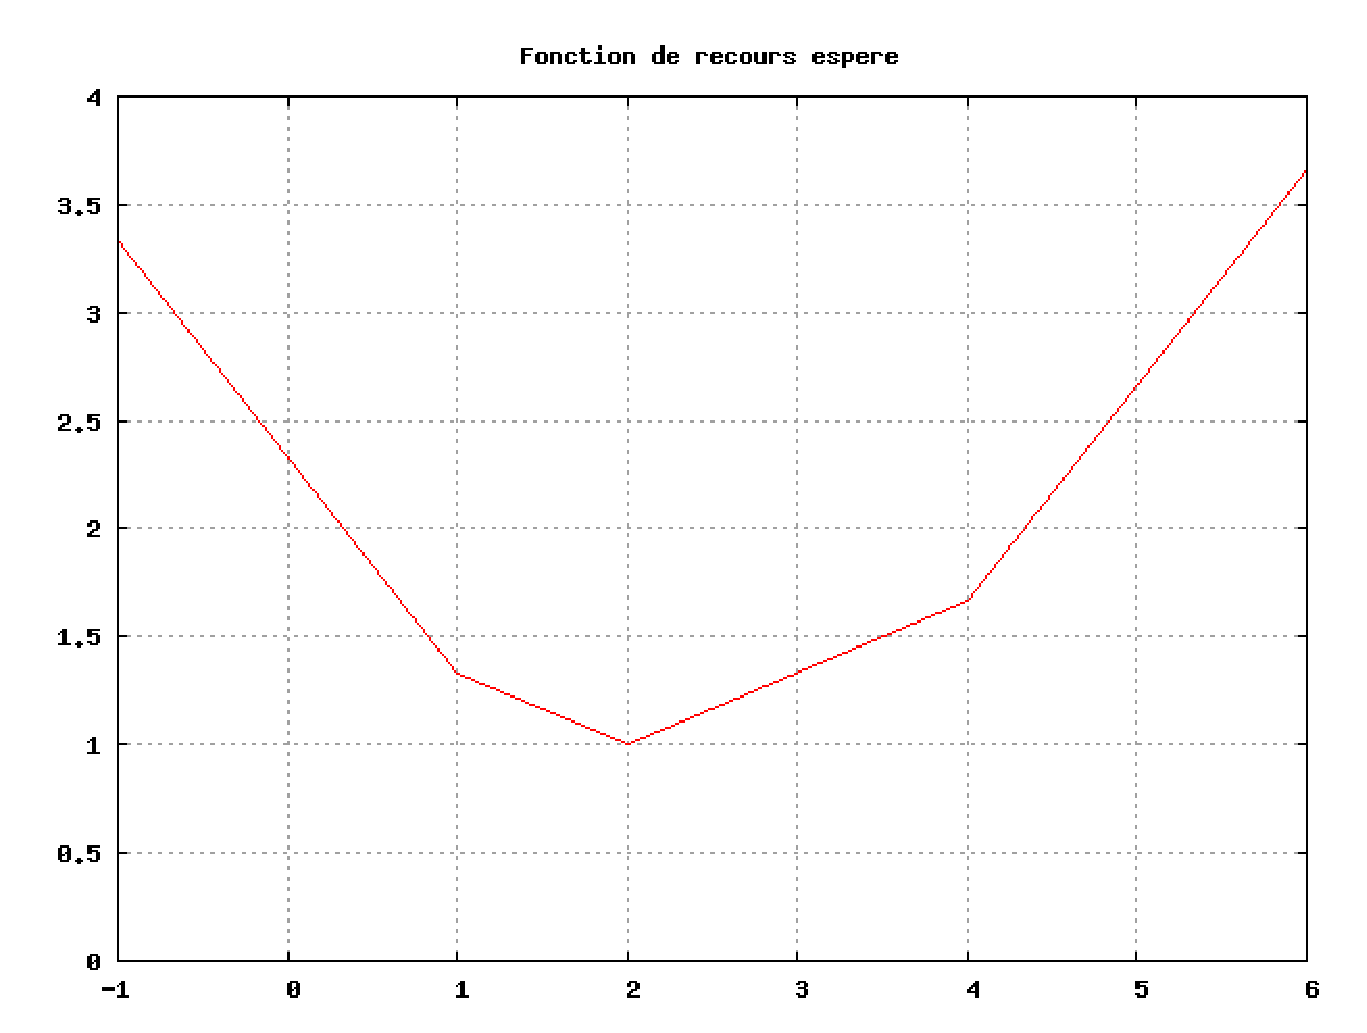
\includegraphics[width=0.9\textwidth]{all.eps}
	
\end{frame}

\begin{frame}
	\frametitle{$\mathcal{Q}(x)$, addition of the cut $\theta \geq 7/3-x$}
	
	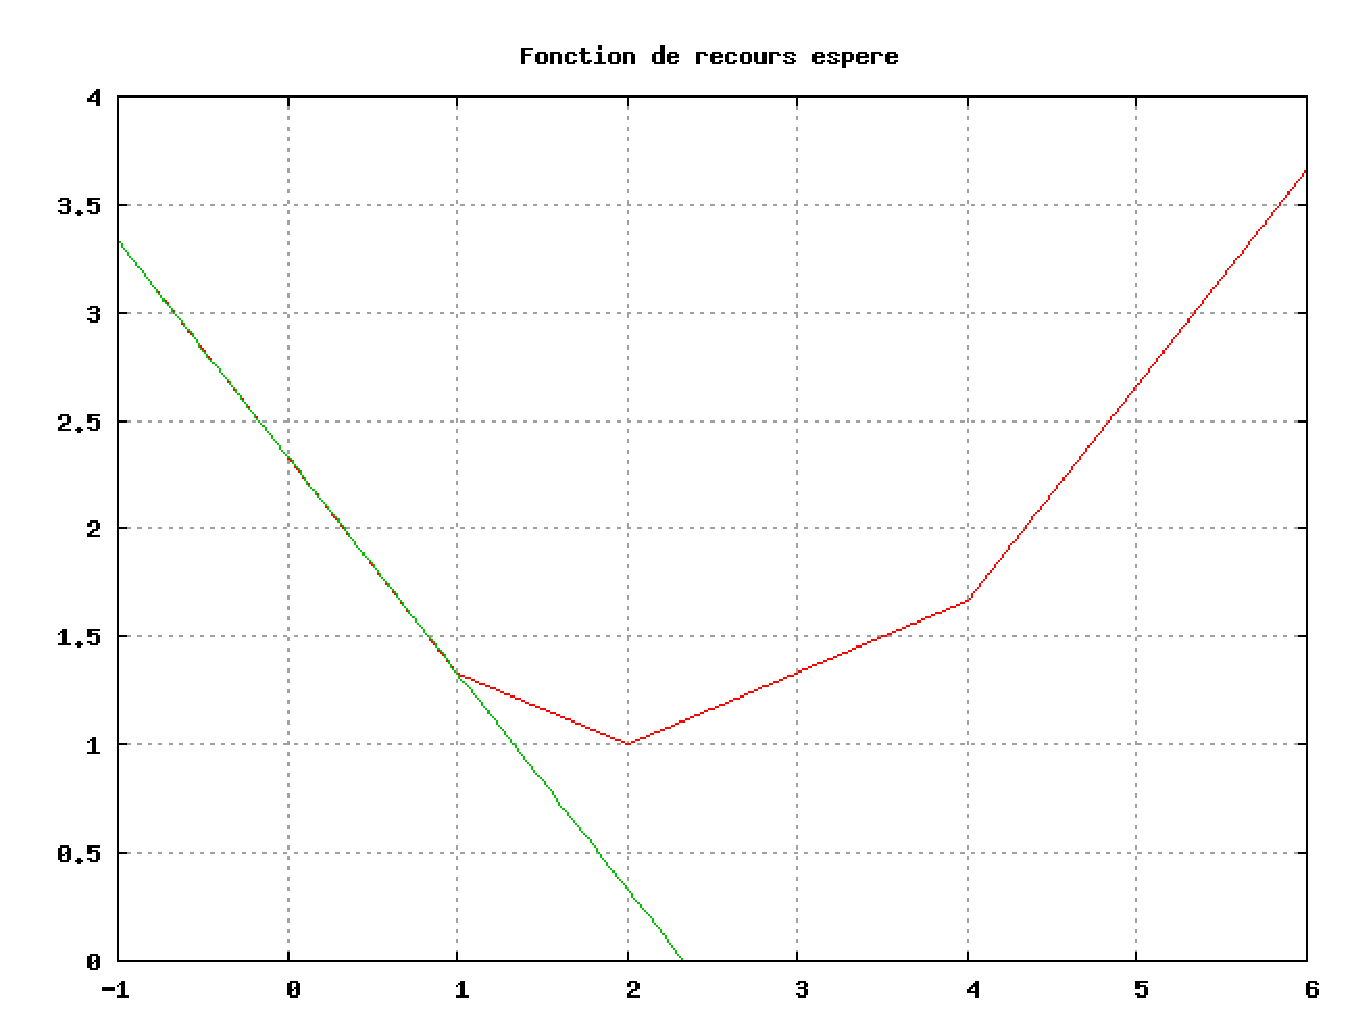
\includegraphics[width=0.9\textwidth]{coupe_1.eps}
	
\end{frame}

\begin{frame}
	\frametitle{$\mathcal{Q}(x)$, addition of the cut $\theta \geq x-7/3$}
	
	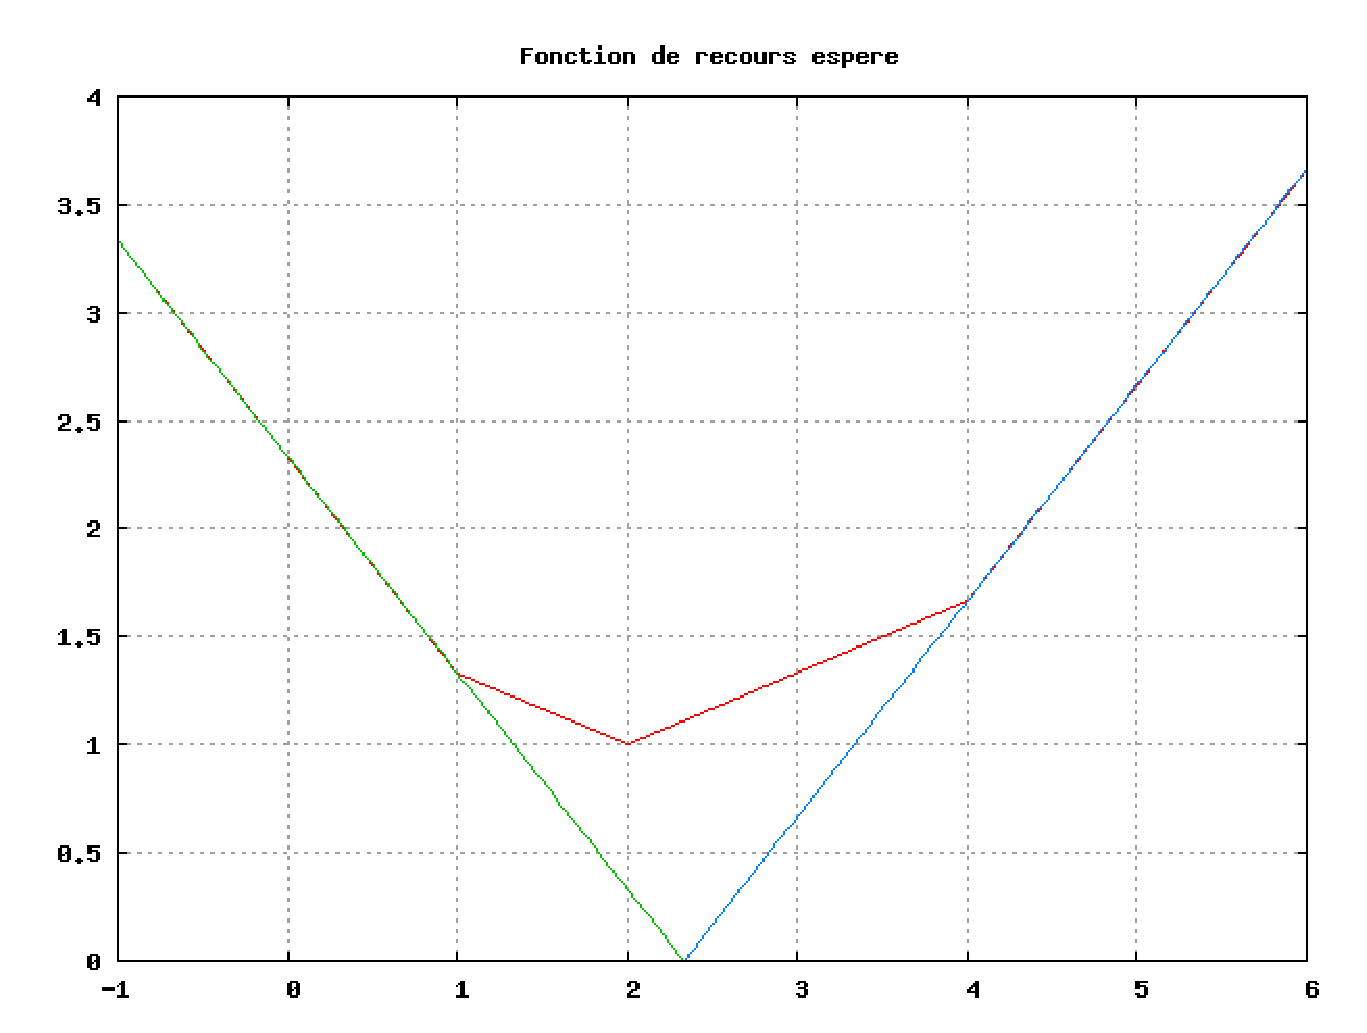
\includegraphics[width=0.9\textwidth]{coupe_2.eps}
	
\end{frame}

\begin{frame}
	\frametitle{$\mathcal{Q}(x)$, addition of the cut $\theta \geq (x+1)/3$}
	
	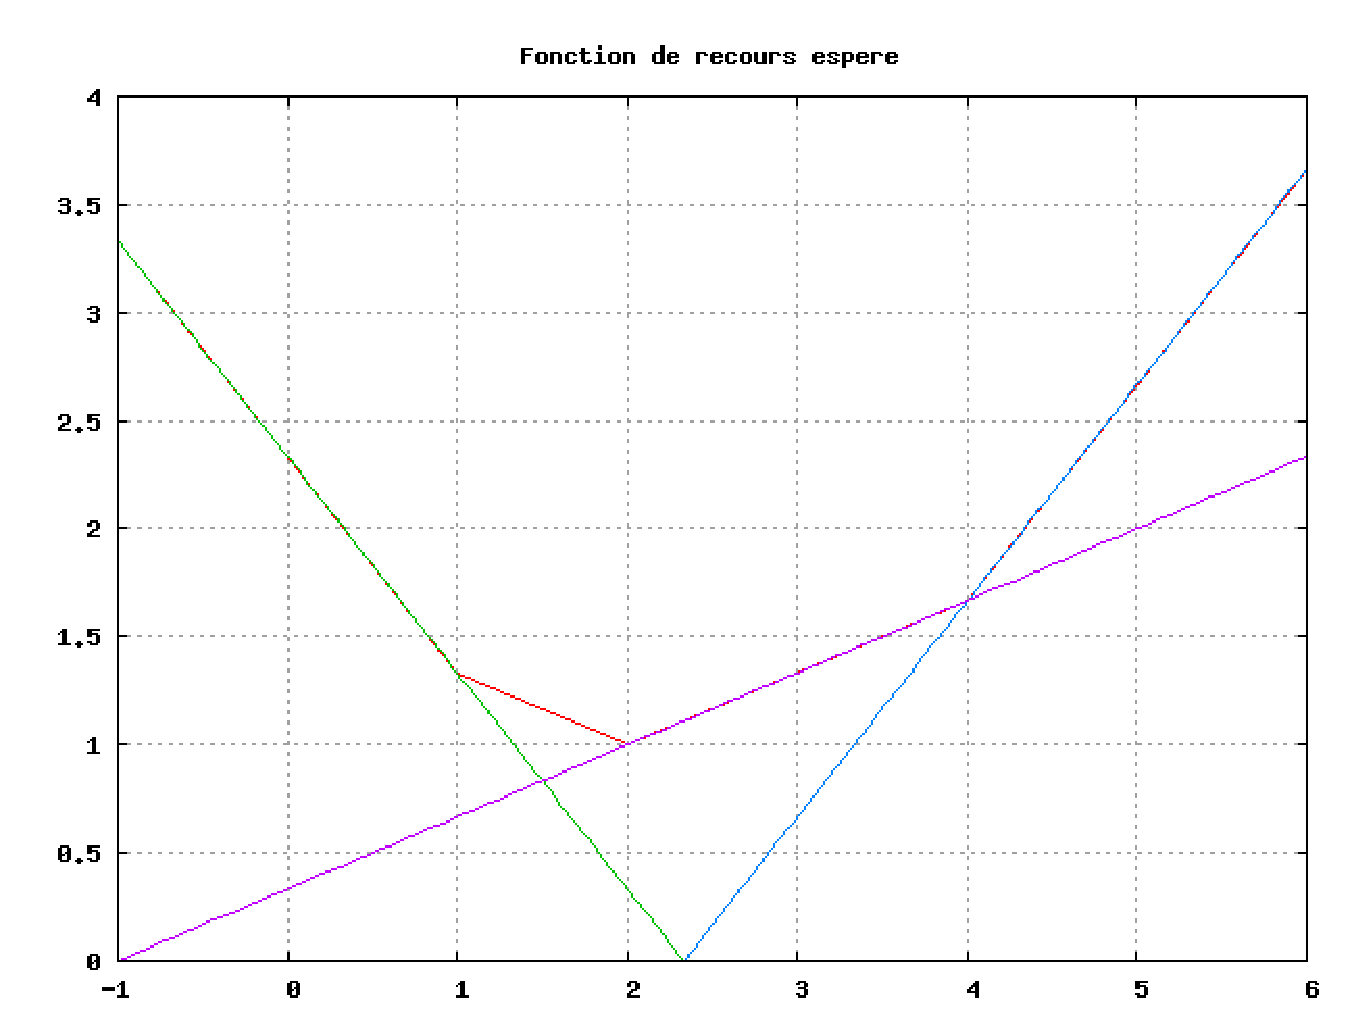
\includegraphics[width=0.9\textwidth]{coupe_3.eps}
	
\end{frame}

\begin{frame}
\frametitle{$\mathcal{Q}(x)$, addition of the cut $\theta \geq (5-x)/3$}
	
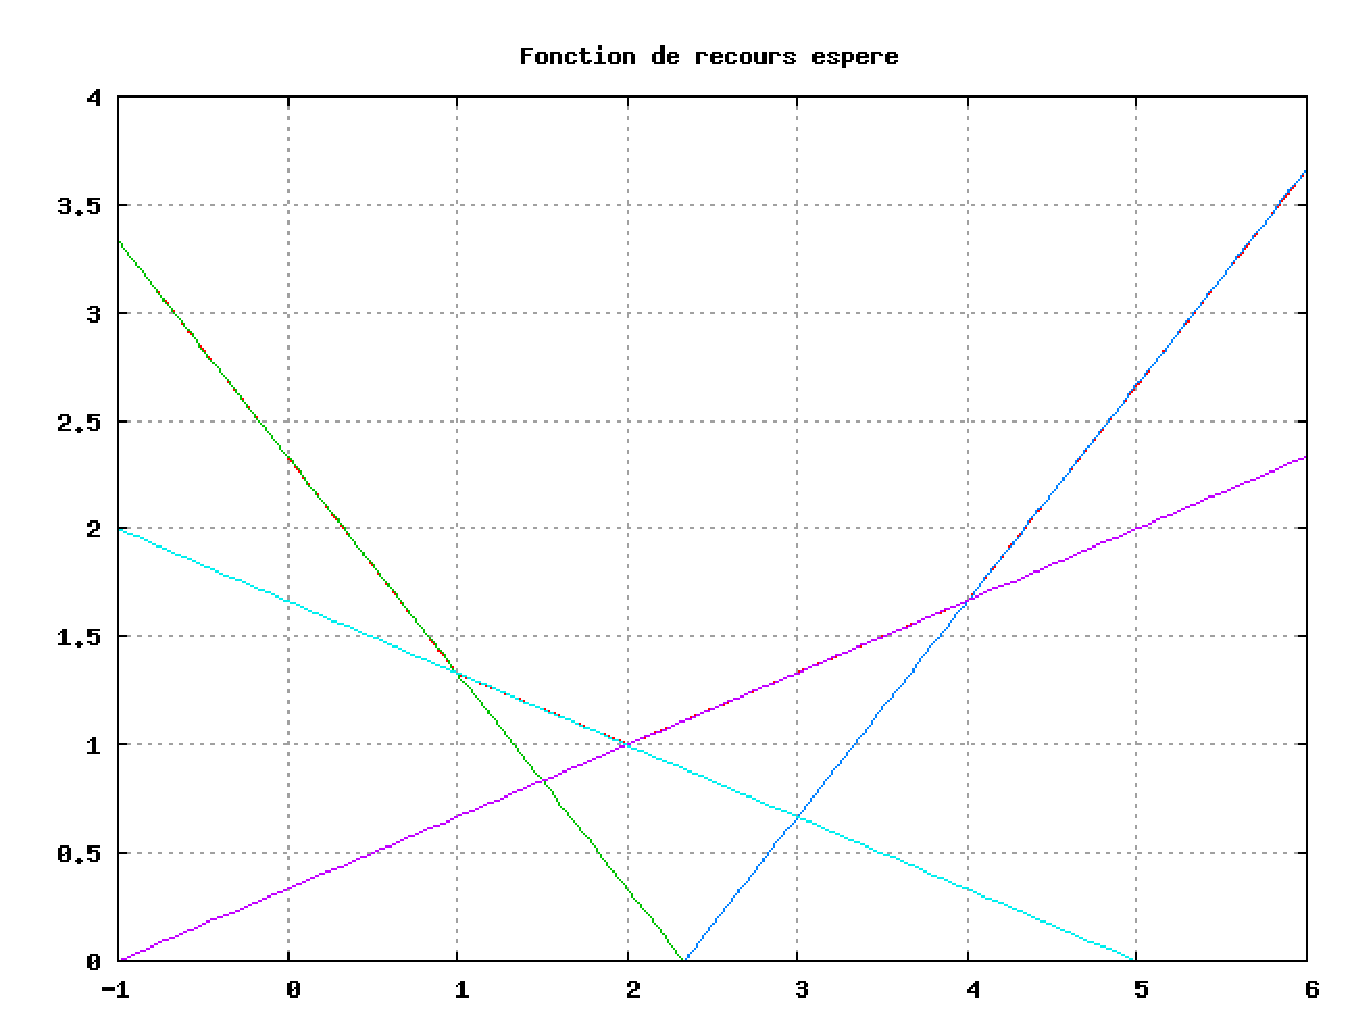
\includegraphics[width=0.9\textwidth]{coupe_4.eps}
	
\end{frame}

\begin{frame}
\frametitle{Multi-cut version}

\begin{itemize}
	\item
	Why do we build one cut only?
	{\red Idea}: approximate {\blue each} $Q(x,\xi_s)$ by an auxiliary variable $\theta_s$, $s \in S$.
	\item
	We new introduce the cuts
	\[
	\theta_s \geq p_s(\hat{\pi}_s)^T(h(\xi_s) - T(\xi_s)x) = \alpha_s +
	\beta_s^Tx,\ s = 1 \in S.
	\]
	In other terms, we keep $|S|$ cuts instead of aggregating them.
	If it is not possible to build these $|S|$ cuts, the solution is optimal.
	\item
	Which method works the best?
	The multi-cut version offers a more detailed information, so in general, we can expect less major iterations, but as more cuts are added, the first-stage program is more expensive to solve.
	As a rule of thumb, the multi-cut approach is more efficient when the number of realizations $S$ is not significantly greater than the number of first-stage constraints.
\end{itemize}

\end{frame}

\begin{frame}
\frametitle{Reminder: subgradients}

Recall that, by {\blue duality},
\[
Q(\hat{x}, \xi_s) =
\max_{\pi} \lbrace \pi^T(h(\xi_s)-T(\xi_s)\hat{x}) \,|\, \pi^TW \leq q(\xi_s)^T) \rbrace.
\]
Therefore, $\exists\ \hat{\pi}$ t.q.
$Q(\hat{x}, \xi_s) = \hat{\pi}^Th(\xi_s)-\hat{\pi}^TT(\xi_s)\hat{x}$.
With respect to the dual variables, we have
\[
Q(x, \xi_s) \geq \hat{\pi}^Th(\xi_s)-\hat{\pi}^TT(\xi_s) x,
\ \forall x \in K_2(\xi_s)
\]
and therefore
\[
Q(x, \xi_s) \geq Q({\hat{x}, \xi_s}) - \hat{\pi}^TT(\xi_s) (x-\hat{x}),
\ \forall x \in K_2(\xi_s).
\]

In other terms, $-T(\xi_s)^T\hat{\pi} \in \partial Q(\hat{x}, \xi_s)$.

\mbox{}

Similarly, by taking the expectation, $- \sum_j p_j T(\xi_j)^T\hat{\pi}_s \in \mathcal{Q}(x)$.

\end{frame}

\begin{frame}
\frametitle{Multicut $L$-shaped method}
	
\begin{description}
\item[Step 0]
With $\theta_s^0$ a lower bound for $Q(x, \xi_s)$, define
\begin{align*}
\mathcal{B}_0 &= \lbrace \rit_n^+ \times \lbrace \theta_1,
\theta_2,\ldots, \theta_{|S|}\rbrace \,|\, Ax = b \rbrace, \\
\mathcal{B}_1 &= \lbrace \rit_n^+ \times \lbrace \theta_1,
\theta_2,\ldots, \theta_{|S|}\rbrace \,|\, \theta_s \geq \theta_s^0,\
\forall s \in S \rbrace.
\end{align*}
Set $\nu = 0$.
\item[Step 1]
Increment $\nu$.
Solve the master problem
\[
\min \left\lbrace c^Tx+\sum_{s \in S} p_s\theta_s \,|\,
(x,\theta_1,\theta_2,\ldots,\theta_{|S|}) \in \mathcal{B}_0 \cap \mathcal{B}_1 \right\rbrace.
\]
Record the solution $( x^{\nu}, \theta_1^{\nu}, \theta_2^{\nu},\ldots,
\theta_{|S|}^{\nu} )$.
\item[Step 2]
Evaluate $\mathcal{Q}(x^{\nu}) = \sum_{s \in S} p_s Q(x^{\nu}, \xi_s)$.
		
		$\mathcal{Q}(x^{\nu}) < \infty$?
\end{description}
	
\end{frame}

\begin{frame}
\frametitle{Multicut $L$-shaped method: step 2}
	
\begin{itemize}
\item
If $\mathcal{Q}(x^{\nu}) = \infty$, there is a realization $\xi_k$ for which $Q(x^{\nu}, \xi_k) = \infty$, we add a feasibility cut and set
\[
\mathcal{B}_1 := \mathcal{B}_1 \cap \lbrace
(x,\theta_1,\theta_2,\ldots,\theta_{|S|}) \,|\, \sigma^T(h(\xi_k) -
T(\xi_k)x) \geq 0\rbrace.
\]
Note: this inequality is the same than in the simple-cut version.\\
Return to Step 1.
\item
If $\mathcal{Q}(x^{\nu}) < \infty$, we are able to solve all the second-stage problems, for all the scenarios, and obtain the corresponding dual solutions $\lambda_s^*$.
We get the subgradients
\[
u = -T_s^T\lambda_s^* \in \partial Q(x^{\nu}, \xi_s).
\]
\end{itemize}
	
\end{frame}

\begin{frame}
\frametitle{Multicut $L$-shaped method: step 2 - $\mathcal{Q}(x^{\nu}) < \infty$}
	
\begin{itemize}
\item
If $Q(x^{\nu}, \xi_s) \leq \theta_s$, $\forall\, s \in S$, stop: $x^{\nu}$ is optimal.
\item
If $Q(x^{\nu}, \xi_s) > \theta_s$,
\[
\mathcal{B}_1 := \mathcal{B}_1 \cap \lbrace (x,\theta_1,\theta_2,\ldots,\theta_{|S|}) \,|\,
\theta_s \geq Q(x^{\nu}, \xi_s) + u^T(x-x^{\nu})\rbrace.
\]
		
Return to Step 1.
\end{itemize}
	
\end{frame}

\begin{frame}
\frametitle{Hybrid approaches}

\begin{itemize}
	\item
	Partition the scenarios in $C$ ``clusters'' $\mathcal{S}_1$,
	$\mathcal{S}_1$, \ldots, $\mathcal{S}_C$, and define
	\[
	\mathcal{Q}_{[\mathcal{S}_k]}(x) = \sum_{s \in \mathcal{S}_k} p_s Q(x, \xi_s).
	\]
	Thus
	\[
	\mathcal{Q}(x) = \sum_{k = 1}^C \mathcal{Q}_{[\mathcal{S}_k]}(x)
	\]
	\[
	-\sum_{s \in \mathcal{S}_k} p_s(T(\xi_s))^T\hat{\pi}_s
	\in \partial \mathcal{Q}_{[\mathcal{S}_k]}(x).
	\]
	\item
	We can therefore do the same: approximate $\mathcal{Q}_{[\mathcal{S}_k]}(x)$ with the subgradient inequality.
\end{itemize}

\end{frame}

\begin{frame}
\frametitle{Algorithm}

\begin{description}
\item[Step 0]
Let $\theta_k^0$ be a lower bound for $\mathcal{Q}_{[\mathcal{S}_k]}(x)$.
Set
\begin{align*}
\mathcal{B}_0 &= \lbrace \rit_n^+ \times \lbrace \theta_1,
\theta_2,\ldots, \theta_C \rbrace \,|\, Ax = b \rbrace, \\
\mathcal{B}_1 &= \lbrace \rit_n^+ \times \lbrace \theta_1,
\theta_2,\ldots, \theta_C \rbrace \,|\, \theta_k \geq \theta_k^0 \rbrace.
\end{align*}
Set $\nu = 0$.
\item[Step 1]
Increment $\nu$ and solve the {\blue master problem}
\[
\min c^Tx + \sum_{k = 1}^C \theta_k \mbox{ t.q. } (x, \theta_1,
\theta_2,\ldots,  \theta_C) \in \mathcal{B}_0 \cap \mathcal{B}_1.
\]
Let $(x^{\nu}, \theta_1^{\nu}, \theta_2^{\nu},\ldots,
\theta_C^{\nu})$ be the found solution.
\end{description}

\end{frame}

\begin{frame}
\frametitle{Algorithm - Step 2}

\begin{itemize}
\item
Evaluate $\mathcal{Q}(x^{\nu}) = \sum_{s \in S} p_s Q(x^{\nu}, \xi_s)$.
\item
If $\mathcal{Q}(x^{\nu}) = \infty$, there is some $\xi_k$ such that $Q(x^{\nu}, \xi_k) = \infty$.
We add a {\red feasibility cut}:
\[
\mathcal{B}_1 := \mathcal{B}_1 \cap \left\lbrace (x, \theta) \,|\,
\sigma^T(h(\xi_k)-T(\xi_k)x) \leq 0 \right\rbrace.
\]
This inequality has no term in $\theta_s$; it is the same inequality than in the standard L-Shaped method.

Go back to Step 1.
\item
If $\mathcal{Q}(x^{\nu}) < \infty$, the $S$ LP's corresponding to the $S$ scenarios can be solved, with the dual solutions $\pi_s^{\nu}$, and
\[
u_k := -\sum_{s \in \mathcal{S}_k} p_s(T(\xi_s))^T\hat{\pi}_s
\in \partial \mathcal{Q}_{[\mathcal{S}_k]}(x).
\]
If $\mathcal{Q}_{[\mathcal{S}_k]}(x) \leq \theta_k$, $k = 1,\ldots,C$, stop: $x^{\nu}$ is optimal.
\end{itemize}

\end{frame}

\begin{frame}
\frametitle{Algorithm - Step 2 (cont'd)}

For each $k$ such that  $\mathcal{Q}_{[\mathcal{S}_k]}(x) >
\theta_k$, add an optimality cut:
\[
\mathcal{B}_1 := \mathcal{B}_1 \cap \left\lbrace (x, \theta_1,
\theta_2,\ldots, \theta_C) \,|\, \theta_k \geq
\mathcal{Q}_{[\mathcal{S}_k]}(x^{\nu}) + u_k^T(x-x^{\nu}) \right\rbrace.
\]

%\mbox{}

%Ok, all right,\ldots but what happens if we start from the optimal solution $x^*$?

\end{frame}

\begin{frame}
\frametitle{Example}

{\red Birge and Louveaux, Section~5.1, Exercice 5., page 200}

\mbox{}

Assume $n_1 = 1$ (dimension of $x$), $m_1 = 0$ (no first-stage constraint), $m_2 = 3$ (three second-stage constraints), $n_2 = 6$ (dimension of $y$), and
\[
W = \begin{pmatrix}
1 & -1 & -1 & -1 & 0 & 0 \\
0 & 1 & 0 & 0 & 1 & 0 \\
0 & 0 & 1 & 0 & 0 & 1
\end{pmatrix}.
\]
Assume moreover $S = 2$, and that the two realizations of $\bxi$ have the same probability.
These realizations are
\begin{align*}
\xi^1 &= (q^1, h^1, T^1)^T, \\
\xi^2 &= (q^2, h^2, T^2)^T.
\end{align*}

\end{frame}

\begin{frame}
\frametitle{Example (cont'd)}

Assume
\begin{align*}
& q^1 = (1,0,0,0,0,0)^T,\ q^2 = (3/2, 0, 2/7, 1, 0, 0)^T, \\
& h^1 = (-1,2,7)^T,\ h^2 = (0,2,7)^T, \\
& T^1 = T^2 = (1,0,0)^T.
\end{align*}

\mbox{}

For the first value $\xi^1$, we have thus the second-stage program
\begin{align*}
\min_y\ & y_1 \\
\mbox{s.t. } & y_1 - y_2 - y_3 -y_4 = -1 - x, \\
& y_2 + y_5 = 2, \\
& y_3 + y_6 = 7, \\
& y \geq 0.
\end{align*}

\end{frame}

\begin{frame}
\frametitle{Example (cont'd)}

It is easy to see that, for $\xi^1$,
\[
Q_1(x) = \begin{cases}
-x-1 & \mbox{if } x \leq -1, \\ 0 & \mbox{if } x \geq -1.
\end{cases}.
\]
For the second value of $Q(x,\xi)$, we can show that
\[
Q_2(x) = \begin{cases}
-1.5x & \mbox{if } x \leq 0, \\
0 & \mbox{if } 0 \leq x \leq 2, \\
\frac{2}{7}(x-2) & \mbox{if } 2 \leq x \leq 9, \\
x - 7 & \mbox{if } x \geq 9.
\end{cases}
\]

Assume also that $-20 \leq x \leq 20$ and $c = 0$.

\mbox{}

What are the (expected) properties that we have for $Q_1(x)$ and
$Q_2(x)$?\\
What about the recourse?

\end{frame}

\begin{frame}
\frametitle{Example: $L$-shaped}

Start from $x = -2$. We have the following sequence of iterates
\begin{description}
\item[Iteration 1] $x^1 = -2$, $\theta^1$ is omitted and we add the cut
\[
\theta \geq -0.5 -1.25x.
\]
\item[Iteration 2] $x^2 = 20$, $\theta^2 = -25.5$, new cut:
\[
\theta \geq 0.5x - 3.5.
\]
\item[Iteration 3] $x^3 = 12/7$, $\theta^3 = -37/14$, new cut:
\[
\theta \geq= 0.
\]
\item[Iteration 4] $x^4 \in [-2/5, 7]$, $\theta^4$.
If $x^4$ is chose as any value in $[0,2]$, stop.
\end{description}

\end{frame}

\begin{frame}
\frametitle{Example: multicut $L$-shaped}

The multicut approach would give the following sequence.
\begin{description}
\item[Iteration 1] $x^1 = -2$, $\theta^1$ and $\theta^2$ are omitted;
we add the cuts $\theta_1 \geq -0.5 - 0.5x,\ \theta_2 \geq -3/4x$.
Note: $\theta_1 \geq \frac{1}{2} (-x-1)$ and $\theta_1 \geq \frac{1}{2} (-1.5x)$
\item[Iteration 2] $x^2 = 20$, $\theta_1^2 = -10.5$, $\theta_2^2 =
-15$; new cuts: $\theta_1 \geq 0$, $\theta_2 \geq 0.5x - 3.5$.
\item[Iteration 3] $x^3 = 2.8$, $\theta_1^3 = 0$, $\theta_2^3 = -2.1$;
new cut: $\theta_2^3 \geq 1/7(x-2)$.
\item[Iteration 4] $x^4 = 0.32$, $\theta_1^4 = 0$, $\theta_2^4 =
-0.24$; new cut: $\theta_2 \geq 0$.
\item[Iteration 5] $x^5 = 0$, $\theta_1^5 = \theta_2^5 = 0$. Stop.
\end{description}

\mbox{}

This example shows the the multicut approach can sometimes take more iterations than the single cut version.

\end{frame}

\begin{frame}
\frametitle{Regularization}

The $L$-shaped method suffers from ``stability'' issues,
\begin{itemize}
\item
especially during the first iterations when we do not have a good model of $\mathcal{Q}(x)$;
\item
especially when we start from a good estimate of the solution.
\end{itemize}
It is therefore useful to {\red regularize} the method. Various techniques exist.

\mbox{}

{\blue Some references} on the stabilization of the Benders decomposition:
\begin{itemize}
\item
Marsten, Hogan, Blankenship (1975);
\item
Lemaréchal (1975,\ldots);
\item
Kiwiel (1983,\ldots);
\item
Neame, Boland, and Ralph (1998).
\end{itemize}

\end{frame}

\begin{frame}
\frametitle{Regularization of the $L$-Shaped method}

\vspace*{-3mm}

\begin{itemize}
\item
{\blue Penalization of the step length}: A. Ruszczy\'nski, {\sl A
Regularized Decomposition for Minimizing a Sum of Polyhedral
Functions}, Mathematical Programming 35, pp. 309--333, 1986.
\item
{\blue Approach in $\|\cdot\|_\infty$}: J. T. Linderoth and S. J. Wright, {\sl
Implementing a Decomposition Algorithm for Stochastic Programming on a
Computational Grid}, Computational Opimization and Applications 24,
pp. 207--250, 2003.
\end{itemize}

\end{frame}

\begin{frame}
\frametitle{Penalization of the step length}

At iteration $k$, we solve the program
\[
\min_x c^Tx + \sum_{j \in C} \theta_j + \frac{1}{2\rho} \| x-x_k \|^2.
\]
\begin{itemize}
\item
Large $\rho$: as the $L$-shaped.
\item
Small $\rho$: we do not move a lot.
\end{itemize}
We speak of {\blue regularized decomposition method}.

\end{frame}

\begin{frame}
\frametitle{Trust-region approach}

The principle is also to penalize the step length.
At iteration $k$, we require $\| x-x_k \|_k \leq \Delta_k$, where $\| \cdot \|_k$ designs an usual norm (typically 2 or $\infty$).

\begin{itemize}
\item
Big $\Delta_k$: as the $L$-shaped.
\item
Small $\Delta_k$: we do not move a lot.
\end{itemize}

We speak of the {\blue trust-region regularization}.

\mbox{}

In both case, we see the introduction of {\blue nonlinear programming} concepts.

\end{frame}

\begin{frame}
\frametitle{Summary}

Let $m(x)$ be the "model" used as first-stage problem.
\begin{itemize}
\item
{\red Multicut $L$-shaped}
\[
m(x) = \min_x \Big\lbrace c^Tx + \sum_{k = 1}^S \theta_k \,|\, (x, \theta_1,
\theta_2,\ldots, \theta_C) \in \mathcal{B}_0 \cap \mathcal{B}_1
\Big\rbrace.
\]
\item
{\red Trust-region}
\begin{align*}
m(x)
= \min_x \Big\lbrace &  c^Tx + \sum_{k = 1}^C \theta_k \,|\, (x, \theta_1,
\theta_2,\ldots, \theta_C) \in \mathcal{B}_0 \cap \mathcal{B}_1, \\
& \| x-x^l \|_{\infty} \leq \Delta_l \Big\rbrace.
\end{align*}
\item
{\red Regularized decomposition}
\begin{align*}
m(x) = \min_x \Big\lbrace & c^Tx + \sum_{k = 1}^C \theta_k + (1/2\rho_l)
\| x-a^l \|_2^2 \\ & \mbox{s.t. } (x, \theta_1, \theta_2,\ldots,
\theta_C) \in \mathcal{B}_0 \cap \mathcal{B}_1, \Big\rbrace.
\end{align*}
\end{itemize}

\end{frame}

\begin{frame}
\frametitle{Regularized decomposition method}

{\red Reference: Birge and Louveaux, Section~5.2}. Multicut version.

\begin{description}
\item[Step 0]
Set $\rho = 1$, $r = \nu = 0$, $s(k) = 0$ for all $k = 1,\ldots,S$.
Select a feasible solution $a^1$.
\item[Step 1]
Set $\nu := \nu+1$, and solve the regularized master program
\begin{align*}
\min\ & c^Tx + \sum_{k = 1}^S \theta_k + \frac{1}{2\rho} \| x - a^{\nu}
\|^2,\\
\mbox{s.t. } & Ax = b,\\
& D_{\ell}^Tx \geq d_{\ell},\ \ell = 1,\ldots,r, \\
& -\beta^T_{\ell(k)} x + \theta_k \geq \alpha_{\ell(k)},\ \ell(k) =
1,\ldots,s(k),\\
& x \geq 0.
\end{align*}
\end{description}

\end{frame}

\begin{frame}
\frametitle{Regularized decomposition method (cont'd)}

\begin{description}
\item[Step 1] (cont'd)
Let $(x^{\nu}, \theta^{\nu})$ be an optimal solution of this program, where $(\theta^{\nu})^T = (\theta^{\nu}_1,\ldots,\theta^{\nu}_K)^T$.

If $s(k) = 0$ for some $k$, $\theta_k^{\nu}$ is ignored in the computation.
If $c^Tx^{\nu} + e^T\theta^{\nu} = c^Ta^{\nu} + \mathcal{Q}(a^{\nu})$, stop: $a^{\nu}$ is optimal.
\item[Step 2]
If a feasibility cut is generated, set $a^{\nu+1} = a^{\nu}$
(unfeasible null step), and return to Step 1.
\item[Step 3]
For $k = 1,\ldots,S$, solve the linear subproblem
\begin{align*}
\min_y &\ q_k^Ty \\
\mbox{s.t. } & Wy = h_k - T_kx^{\nu}, \\
& y \geq 0.
\end{align*}
Compute $\mathcal{Q}_k(x^{\nu})$.
\end{description}

\end{frame}

\begin{frame}
\frametitle{Regularized decomposition method (cont'd)}

\begin{description}
\item[Step 3] (cont'd) If
\[
\theta_k^{\nu} < p_k (\pi_k^{\nu})^T(h_k - T_kx^{\nu}),
\]
add an optimality cut of the form
\[
-\beta^T_{\ell(k)} x + \theta_k \geq \alpha_{\ell(k)}.
\]
Set $s(k) = s(k)+1$.
\item[Step 4] If for all $k$,
\[
\theta_k^{\nu} \geq p_k (\pi_k^{\nu})^T(h_k - T_kx^{\nu}),
\]
set $a^{\nu+1} := x^{\nu}$ (exact serious step). Return to Step 1.
\end{description}

\end{frame}

\begin{frame}
\frametitle{Regularized decomposition method (cont'd)}

\begin{description}
\item[Step 5] If
\[
c^Tx^{\nu} + \mathcal{Q}(x^{\nu}) \leq c^Ta^{\nu} + \mathcal{Q}(a^{\nu}),
\]
set $a^{\nu+1} := x^{\nu}$ (serious approximative step).

Otherwise, set $a^{\nu+1} := a^{\nu}$.

Return to Step 1.
\end{description}

\mbox{}

{\blue Immediate extension}: allow $\rho$ to vary.

\mbox{}

The implementation of the regularized $L$-shaped raises various practical questions.
An efficient implementation is proposed in Ruszczy\'nski (1986).
\end{frame}

\begin{frame}
\frametitle{Example: regularized $L$-shaped}

Take $a^1 = -0.5$ as starting point.
This point corresponds to the solution of the expected value problem. i.e the problem obtained by replacing $\bxi$ by $E[\xi]$.
The second stage program becomes
\begin{align*}
\min\ & \frac{5}{4}y_1 + \frac{1}{7}y_3 + \frac{1}{2}y_4\\
\mbox{s.t. } & y_1 - y_2 - y_3 - y_4 = -\frac{1}{2}-x, \\
& y_2+y_5 = 2, \\
& y_3+y_6 = 7, \\
& y \geq 0.
\end{align*}

\mbox{}

\mbox{}

{\blue Exercise}: check that $a^1 = -0.5$ is indeed the optimal value of this program (using the KKT/primal-dual conditions).
\end{frame}

\begin{frame}
\frametitle{Example: regularized $L$-shaped (cont'd)}

For $a^1 = -0.5$, the regularized master problem has also for solution $x^1 = -0.5$, and the second stage program of the expected-value problem has the solution $(0,0,0,0,2,7)$, while $Q_1(a^1) = 0$, $Q_2(a^1) = 3/4$, so $\mathcal{Q}(a^1) = 3/8$.
The regularized approach leads to the following iterations.
\begin{description}
\item[Iteration 1] The cuts $\theta_1 \geq 0$, $\theta_2 \geq -3/4
x$ are added. $a^2:= a^1$.
\item[Iteration 2]
The regularized master program is
\begin{align*}
\min\ & \theta_1 + \theta_2 + \frac{1}{2}(x+0.5)^2 \\
\mbox{s.t. } & \theta_1 \geq 0,\ \theta_2 \geq -\frac{3}{4}x,
\end{align*}
with the solution $x^2 = 0.25$, $\theta_1 = 0$, $\theta_2 = -3/16$.
A new cut $\theta_2 \geq 0$ is added.
As $\mathcal{Q}(0.25) = 0 < \mathcal{Q}(a^1)$, $a^3 := 0.25$ (serious approximate step).
\end{description}
\end{frame}

\begin{frame}
\frametitle{Example: regularized $L$-shaped (cont'd)}

\begin{description}
\item[Iteration 3]
The regularized master problem is
\begin{align*}
\min\ & \theta_1 + \theta_2 + \frac{1}{2}(x-0.25)^2 \\
\mbox{s.t. } & \theta_1 \geq 0,\ \theta_2 \geq -\frac{3}{4}x, \theta_2
\geq 0,
\end{align*}
with the solution $x^3 = 0.25$, $\theta_1 = 0$, $\theta_2 = 0$.
As $\theta^{\nu} = \mathcal{Q}(a^{\nu})$, a solution is found.
\end{description}

\begin{theo}
If the original problem has a solution, the algorithm stops after a finite number of iterations.
Otherwise, it generates a sequence of feasible points $\lbrace a^{\nu} \rbrace$ such that
$\mathcal{Q}(a^{\nu}) \rightarrow -\infty$, as $\nu \rightarrow \infty$.
\end{theo}
\begin{proof}
See Birge and Louveaux, Section~5.2.
\end{proof}
\end{frame}

\begin{frame}
\frametitle{Regularization using trust-region methods}

The basic philosophy of trust-region methods is to replace the original problem with some locally valid approximation easier to handle.

\mbox{}

Here, our original problem is
\begin{align*}
\min_x \ & c^T x + \cQ(x) \\
\mbox{s.t. } & Ax = b \\
& x \geq 0.
\end{align*}
The model is
\begin{align*}
\min_x \ & m(x) := c^T x + \theta \\
\mbox{s.t. } & Ax = b \\
& {\rm feasibility\ cuts} \\
& {\rm optimality\ cuts} \\
& x \geq 0.
\end{align*}
\end{frame}

\begin{frame}
\frametitle{Regularization using trust-region methods (cont'd)}

Since the model is only valid locally, we constraint the next iterate to remain in a trust region centered at the current solution $x_k$, where $k$ is the iteration index.
The trust region is defined by
$$
\cB_k = \{ x \,|\, \| x-x_k \|_k \leq \Delta_k \},
$$
where $\Delta_k$ is the trust-region radius, and $\|\cdot\|_k$ is the norm used at iteration $k$.
In the context a linear programming, it is common to use $\infty$-norm as they correspond to bound constraints.
The trust-region subproblem at iteration $k$ is now
\begin{align*}
\min_{x,\theta} \ & m(x) := c^T x + \theta \\
\mbox{s.t. } & Ax = b \\
& {\rm feasibility\ cuts} \\
& {\rm optimality\ cuts} \\
& \|x-x_k\|_{\infty} \leq \Delta_k,\ x \geq 0.
\end{align*}
\end{frame}

\begin{frame}
\frametitle{Regularization using trust-region methods (cont'd)}

Let $x^*$ be the first-stage solution.
We can compare the model reduction with the original problem reduction, by computing the ratio
\begin{align*}
\rho = \frac{c^T(x_k-x^*)+\cQ(x_k)-\cQ(x^*)}{m(x_k)-m(x^*)}
\end{align*}

\mbox{}

If $\rho$ is too small (for instance $\rho < \eta_1 < 1$), set $x_{k+1} = x_k$ and set $\Delta_{k+1} < \Delta_k$.
Otherwise, set $x_{k+1} = x^*$.\\

\mbox{}

If $\rho \geq \eta_2 \geq \eta_1$, choose $\Delta_{k+1} \in [\Delta_k, +\infty]$.

\mbox{}

Note: additional details and considerations in Linderoth and Wright.

\end{frame}

\end{document}